% This is samplepaper.tex, a sample final report template.
% The template is based on Springer's LNCS template.
%
% Version 1.00 of 2018/08/01
%
% This format follows departmental guideline: 11pt, double space, single column.
% For capstone requirement, your report should be 20+ pages of length. 
% This *excludes* the list of references (bibliography section) in this format. 
% Only the main content counts toward the 20 pages.
%
% A guideline for breakdown of your final report (20 pages) would be like following:
%   2 pages: introduction, verbal problem statement, list of contributions
%   3 pages: related literature survey, prior works, comparison to proposing method
%   1 page: problem definition, notations (can be merged to proposing methods section)
%   5-6 pages: proposing methods
%   7-8 pages: experiment design, results, analysis
%   1 pages: conclusion, future works
% The page breakdown will be adjusted based on the number of units you are taking.
% If you are taking 0.5 units (10 pages), all page breakdown above will also reduce to half as:
%   1 pages: introduction, verbal problem statement, list of contributions
%   1.5 pages: related literature survey, prior works, comparison to proposing method
%   0.5 page: problem definition, notations (can be merged to proposing methods section)
%   2.5-3 pages: proposing methods
%   3.5-4 pages: experiment design, results, analysis
%   0.5 pages: conclusion, future works
% If you are taking 0.25 units (5 pages), they will become a quarter of the ones above as:
%   1 pages: introduction, verbal problem statement, list of contributions
%   1 pages: related literature survey, prior works, comparison to proposing method
%   0.25 page: problem definition, notations (can be merged to proposing methods section)
%   1 pages: proposing methods
%   1.5 pages: experiment design, results, analysis
%   0.25 pages: conclusion, future works
%
\RequirePackage{amsmath} % a cumbersome thing to use AMS in Spring document class.
\documentclass[runningheads,11pt]{llncs_bigfont_absbib}
\usepackage{geometry} \geometry{margin=1in}
%
% When done with your draft, try to comment out the following command and see if
% your report has required length. For example, for capstone, you should see at least
% 10 full pages in single space. For submission, put the double spacing option back 
% and make your PDF in 20 pages.
\usepackage{setspace} \doublespacing
%
\usepackage{graphicx,wrapfig,lipsum}
\usepackage{epstopdf}
% Used for displaying a sample figure. If possible, figure files should
% be included in EPS format.
%
% If you use the hyperref package, please uncomment the following line
% to display URLs in blue roman font according to Springer's eBook style:
% \renewcommand\UrlFont{\color{blue}\rmfamily}
\usepackage[utf8]{inputenc}
\usepackage{titleps}
\usepackage{amssymb}
\usepackage{amsfonts}
\usepackage{comment}
\usepackage{bm}
\usepackage[linesnumbered,ruled]{algorithm2e}
\usepackage[caption=false]{subfig}
\usepackage{color}
\usepackage{fancyhdr}
\usepackage{adjustbox}
\usepackage{url}
\usepackage{enumitem}
%testing to fix the bar chart issue
\usepackage{tikz}
\usepackage{pgfplots}
\usepackage{pgfplotstable}
\pgfplotsset{compat=1.18}
\usetikzlibrary{calc}

% handy macro for argmin and argmax in optimization related math
\DeclareMathOperator*{\argmin}{arg\,min}
\DeclareMathOperator*{\argmax}{arg\,max}

\begin{document}
%
\title{A Comparative Study of SLAM Algorithms
\\ % use this to start a new line
for Robot Operating System (ROS)}
%
%\titlerunning{Abbreviated paper title}
% If the paper title is too long for the running head, you can set
% an abbreviated paper title here
%
\author{Stenneth Swaby}
%
\authorrunning{S. Swaby}
% First names are abbreviated in the running head.
% If there are more than two authors, 'et al.' is used.
%
\institute{The College of New Jersey, Ewing NJ 08628, USA
\\
\email{swabys1@tcnj.edu}}
%
\maketitle              % typeset the header of the contribution
%
\begin{abstract}
Loop closure remains one of the most persistent open challenges in mobile robotics and SLAM (Simultaneous Localization and Mapping). A system cannot robustly detect loop closure unless the underlying algorithm consistently produces maps that closely match the environment's actual structure. Therefore, determining which SLAM algorithm generates the most accurate and repeatable representation of a known environment is a critical prerequisite for improving long-term autonomy. In this study, a TurtleBot3 platform equipped with a 2D LiDAR sensor was manually teleoperated through a controlled test environment constructed from cardboard boxes. This environment, referred to as the Maze, served as the ground truth; its real-world dimensions were carefully measured before experimentation, so that all generated occupancy grids could be compared against a fixed, known layout.
Two widely used ROS2 SLAM algorithms, Google Cartographer and SLAM Toolbox, were evaluated under identical conditions. Each algorithm was run multiple times while the robot followed the same prescribed path through the Maze, allowing for assessment of mapping consistency in addition to mapping accuracy. After collection, all generated maps were saved using ROS2’s map server tools, normalized to a common pixel resolution, and aligned to the ground-truth reference. A custom Python pipeline was developed to overlay the maps and compute quantitative error metrics, including per-pixel map error, variance, and correlation with the ground truth.
The results demonstrate significant differences in map quality between the two algorithms, highlighting the importance of selecting the appropriate algorithm when addressing higher-level SLAM challenges, such as loop closure. By identifying which algorithm yields the most accurate baseline map, this work provides foundation-level insight that supports more advanced research into long-duration autonomy, localization drift correction, and robust loop-closure detection in mobile robotic systems.


\keywords{Simultaneous Localization and Mapping (SLAM) \and Occupancy Grid \and Mapping Error \and Robot Operating System (ROS) \and TurtleBot3 \and LiDAR  \and Google Cartographer \and SLAM Toolbox}
\end{abstract}
%
%
%
\section{Introduction}
\subsection{Motivation and Background}
In an increasingly automated world filled with self-driving vehicles, autonomous delivery systems, and household service robots, it is easy to overlook the engineering and algorithmic design that enable these machines to navigate safely and intelligently. Simultaneous Localization and Mapping (SLAM) algorithms form the foundation of this capability by allowing robots to build a map of their environment while estimating their own position within it. Although many companies treat their navigation pipelines as proprietary technology, a large body of open-source SLAM research is available to the academic community. In this paper, I focus on two widely used open-source SLAM frameworks, SLAM Toolbox and Google Cartographer, and compare their ability to produce accurate and consistent maps.
A deep understanding of how SLAM algorithms receive sensor data, process it, and reconstruct the surrounding world is essential for addressing higher-level robotics challenges. One of the most important open problems is loop closure, the ability to recognize previously visited locations and correct accumulated drift. However, before we can meaningfully investigate loop closure, we must first examine a more fundamental issue: which SLAM algorithm can consistently reproduce the actual dimensions of a controlled environment? If an algorithm cannot generate an accurate baseline map, it cannot reliably detect or correct loop closures.
Both of the SLAM algorithms examined in this study come from well-established contributors within the robotics and ROS communities. Google Cartographer was initially developed by Google’s autonomous systems research team and released as an open-source project to support high-accuracy mapping and localization for indoor and outdoor environments. In contrast, SLAM Toolbox was developed by Steve Macenski as part of the ROS2 Navigation project to provide a flexible, long-term-supported SLAM framework specifically designed for robotics research, commercial robotics platforms, and real-time operation in constrained environments.
\subsection{Prior Work and Contributions}
At the start of this research project, I was fortunate to have the opportunity to complete a semester of mentored research under the supervision of Dr. Sejong Yoon. His guidance, combined with extensive documentation provided by ROBOTIS, the developers and suppliers of the TurtleBot3 platform, played an essential role in helping me build a solid foundation in ROS2 and mobile robot navigation. In addition to this formal documentation, the Articulated Robotics ROS2 tutorial series proved instrumental in helping me understand the practical side of working with ROS2, including how to structure packages, launch nodes, visualize data in RViz2, and interpret LiDAR and odometry topics. I also relied heavily on the well-maintained open-source repositories available to the robotics community, including Google’s Cartographer GitHub project and the ROS2 Navigation documentation for SLAM Toolbox developed by Steve Macenski. Together, these resources were essential in helping me understand how each SLAM algorithm operates, how map data is generated, and how the TurtleBot3 integrates its LiDAR and odometry sensors within the ROS2 ecosystem.
Building on this foundational knowledge, I conducted a literature review to identify prior comparative studies of SLAM algorithms. One particularly relevant study was conducted by Li and Zhu, who evaluated the performance of several 2D LiDAR SLAM algorithms in simulated orchard environments \cite{Li2024OrchardSLAM}. Their work provided valuable insights into how different SLAM frameworks perform under varying conditions, such as terrain roughness and sensor configurations. However, their study was limited to simulated environments, which may not fully capture the complexities of real-world scenarios.
To address this gap, my research focuses on a controlled physical environment, referred to as the Maze, constructed from cardboard boxes. This setup allows for precise measurement of the environment's dimensions, providing a reliable ground truth for evaluating mapping accuracy. By manually teleoperating the TurtleBot3 through the Maze and collecting data using both SLAM Toolbox and Google Cartographer, I aim to provide a direct comparison of their mapping performance in a real-world context.

In addition to comparing individual SLAM algorithms, prior research has examined how the choice of map representation influences overall system performance. Most classical 2D SLAM frameworks, including SLAM Toolbox, rely on occupancy grid maps, which discretize the environment into fixed-size grid cells labeled as free, occupied, or unknown. While this representation is computationally efficient and well-suited for real-time navigation, it inherently loses fine structural details due to discretization. Small geometric features become blurred or merged, and subtle variations in wall curvature or obstacle edges are not preserved. In contrast, modern systems often incorporate point cloud representations, which preserve richer geometric information by storing exact coordinate measurements from LiDAR or depth sensors. Google Cartographer adopts a hybrid approach, maintaining a high-resolution point cloud during scan matching while generating an occupancy grid only as the final output. This allows Cartographer to achieve more accurate local scan alignment, though the final occupancy grid remains subject to discretization limits. As noted in the literature, these representational differences can meaningfully affect mapping accuracy, especially in small, structured indoor spaces where fine details matter.

Beyond representation, researchers have emphasized that map accuracy plays a central and foundational role in higher-level robotic functions, including loop closure, localization, and autonomous navigation. Loop-closure algorithms depend on the ability to recognize previously visited locations; even minor geometric distortions in the map can prevent accurate place recognition, leading to persistent drift in the pose graph. Likewise, localization algorithms such as Monte Carlo localization compare incoming sensor measurements with the existing map. If the map is inaccurate, particle convergence becomes unreliable, resulting in poor pose estimates and unstable motion. Navigation pipelines also depend on the fidelity of the occupancy grid: inflated obstacles, shifted walls, or missing structural boundaries can cause planners to generate unsafe, suboptimal, or even infeasible paths. For these reasons, numerous studies, including Li and Zhu’s evaluation of 2D SLAM in orchard environments, stress that accurate and consistent map reconstruction is a prerequisite for robust long-term autonomy. This motivates the present study’s focus on quantitative map-error analysis, which directly assesses the quality of the environmental representation provided by each SLAM algorithm.

\subsection{TurtleBot3 and LiDAR Sensor} 
In this section, I want to take a deeper look at the hardware platform used in this study, the TurtleBot3, and its integrated 2D LiDAR sensor. The TurtleBot3 is a popular open-source robotic platform developed by ROBOTIS, designed for education, research, and prototyping in mobile robotics. I worked on the Burger configuration. It is built on a modular architecture that allows for easy customization and expansion, making it an ideal choice for experimenting with SLAM algorithms. 
The TurtleBot3 platform uses the LDS-01 2D LiDAR sensor, which provides a full 360° planar scan at approximately 300 ± 10 RPM with an angular resolution of 1°. The sensor measures distances from 120 mm up to 3.5 m, making it well-suited for indoor environments but more limited in larger or open spaces. According to manufacturer specifications, its distance accuracy is ±15 mm for short-range measurements (120–499 mm) and ±5 percent for medium-to-long-range measurements (500–3,500 mm). 
Distance precision follows a similar pattern, specified as ±10 mm for short ranges and ±3.5 percent for longer ranges. These values indicate that measurement noise increases as objects move farther from the sensor, and that the 1° angular resolution provides relatively coarse spatial detail compared to modern high-resolution LiDAR systems. 
\cite{ROBOTIS_TB3_Features}

\begin{figure}[!ht]
    \centering
    \subfloat[TurtleBot3 Burger with LDS-01 LiDAR]{
        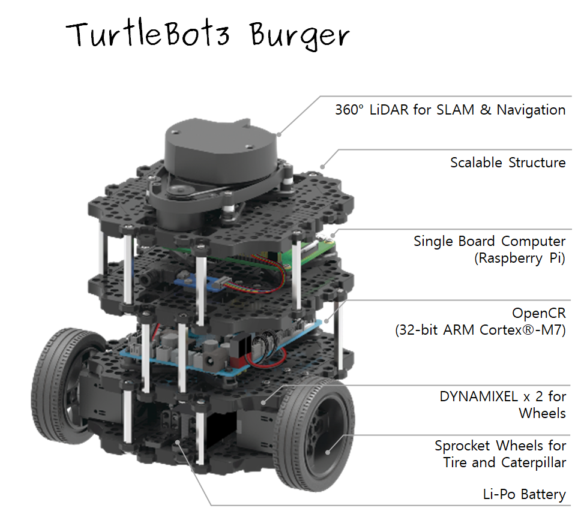
\includegraphics[width=0.45\columnwidth]{images/TurtleBot3_Burger.png}
    }
    \caption{TurtleBot3 Burger platform equipped with LDS-01 2D LiDAR sensor.\cite{ROBOTIS_TB3_Features}}
    \label{fig:subfigname}
\end{figure}

Its core hardware includes a lightweight chassis driven by two Dynamixel servomotors, providing precise wheel control and built-in feedback for velocity and odometry estimation. 
The platform is powered by the OpenCR control board, which integrates a 32-bit ARM microcontroller, inertial measurement unit (IMU), power management, and communication interfaces for ROS2. 
The Burger model also supports expansion through modular plates, allowing users to mount additional sensors, microcontrollers, or compute units such as the Raspberry Pi or NVIDIA Jetson series. 
Despite its small size, it supports full ROS2 navigation capabilities, including teleoperation, autonomous driving, and map generation. However, while these features make the TurtleBot3 a flexible platform, this study does not focus heavily on its general hardware architecture. 
Instead, the emphasis is placed on the integrated 2D LiDAR sensor, as its measurement performance has the most direct influence on mapping quality and therefore plays the central role in the SLAM evaluation conducted in this research.

\section{Experimental Setup and Methodology}
\subsubsection{Required Software and Packages}
To ensure that the results of this study can be repeated under identical conditions, the software and system configuration were kept consistent throughout all experiments. All testing was performed on Ubuntu 22.04, the operating system recommended for ROS2 Humble Hawksbill, which served as the robotics middleware for the TurtleBot3 platform. Both SLAM Toolbox and Google Cartographer were installed from their respective GitHub repositories, following the official installation instructions provided by their developers. SLAM Toolbox was launched using a custom ROS2 launch file written specifically for this study, while Cartographer was executed using the official Cartographer launch procedure outlined in the ROBOTIS TurtleBot3 E-Manual \cite{ROBOTIS_TB3_SlamTab,ROBOTOIS_Cartographer}.
This setup ensured that eachTo ensure that the results of this study can be repeated under identical conditions, the software and system configuration were kept consistent throughout all experiments. All testing was performed on Ubuntu 22.04, the operating system recommended for ROS2 Humble Hawksbill, which served as the robotics middleware for the TurtleBot3 platform. Both SLAM Toolbox and Google Cartographer were installed from their respective GitHub repositories, following the official installation instructions provided by their developers. SLAM Toolbox was launched using a custom ROS2 launch file written specifically for this study, while Cartographer was executed using the official Cartographer launch procedure outlined in the ROBOTIS TurtleBot3 E-Manual \cite{ROBOTIS_TB3_SlamTab,ROBOTOIS_Cartographer}. This setup ensured that each SLAM algorithm operated under the same operating system, ROS2 distribution, sensor configuration,
and execution procedure, which is essential for producing fair and repeatable mapping comparisons. SLAM algorithm operated under the same operating system, ROS2 distribution, sensor configuration, 
and execution procedure, which is essential for producing fair and repeatable mapping comparisons.

\subsubsection{Controlled Environment (The Maze)}
To construct a controlled, repeatable experimental environment, Eric Revera and I designed a physical test space made entirely from cardboard boxes and flat obstacles. Throughout the summer of 2025, we iteratively experimented with several configurations of this environment to determine which layout would provide both a meaningful challenge for the SLAM algorithms and a reliable reference for quantitative analysis. After evaluating multiple designs, we finalized the configuration that served as the Ground Truth for this study. The ground truth refers to the precise, measurable dimensions of the physical environment that the LiDAR sensor measures and that SLAM algorithms aim to reconstruct. Establishing accurate ground truth is essential in mapping studies because it enables each generated map to be evaluated not only qualitatively but also against a fixed, verifiable spatial reference.

The final test environment measured 2.44 meters in length and 1.37 meters in width, forming a rectangular workspace well-suited for indoor mobile robot testing. Four numbered boxes were placed along the interior perimeter, each centered on the middle of a different wall. Box 1, positioned along the left wall, measured 0.39 m × 0.43 m. Box 2, located along the bottom wall, had identical dimensions of 0.39 m × 0.43 m. Box 3 was placed along the right-most wall and measured 0.44 m × 0.24 m, while Box 4, centered along the top wall, measured 0.29 m × 0.24 m. These varying box sizes introduced asymmetry into the environment, providing more distinctive geometric features for the SLAM algorithms to detect and reconstruct.

To minimize risk, control variability, and ensure consistent mapping data across all trials, a fixed navigation path was marked on the floor with painter’s tape. This predefined path was carefully measured so that the TurtleBot3 remained approximately 0.15 meters away from each box at its closest point. The path formed a rectangular loop, encouraging the robot to traverse the entire environment while maintaining consistent proximity to obstacles. During each trial, the TurtleBot3 was manually teleoperated along this route at a constant linear velocity of 0.01 m/s, chosen to reduce inertial effects, prevent wheel slip, and ensure that the LiDAR sensor had sufficient time to collect stable scans. Maintaining identical path direction, speed, and starting pose for every run was essential to ensuring that SLAM Toolbox and Google Cartographer were evaluated under truly comparable, repeatable conditions.
\begin{figure}[!ht] % this controls figure location. h is here, t is top, b is bottom. you can optionally use ! to enforce the layout, e.g. [!ht]
    \centering
        \subfloat[Photographed test environment]{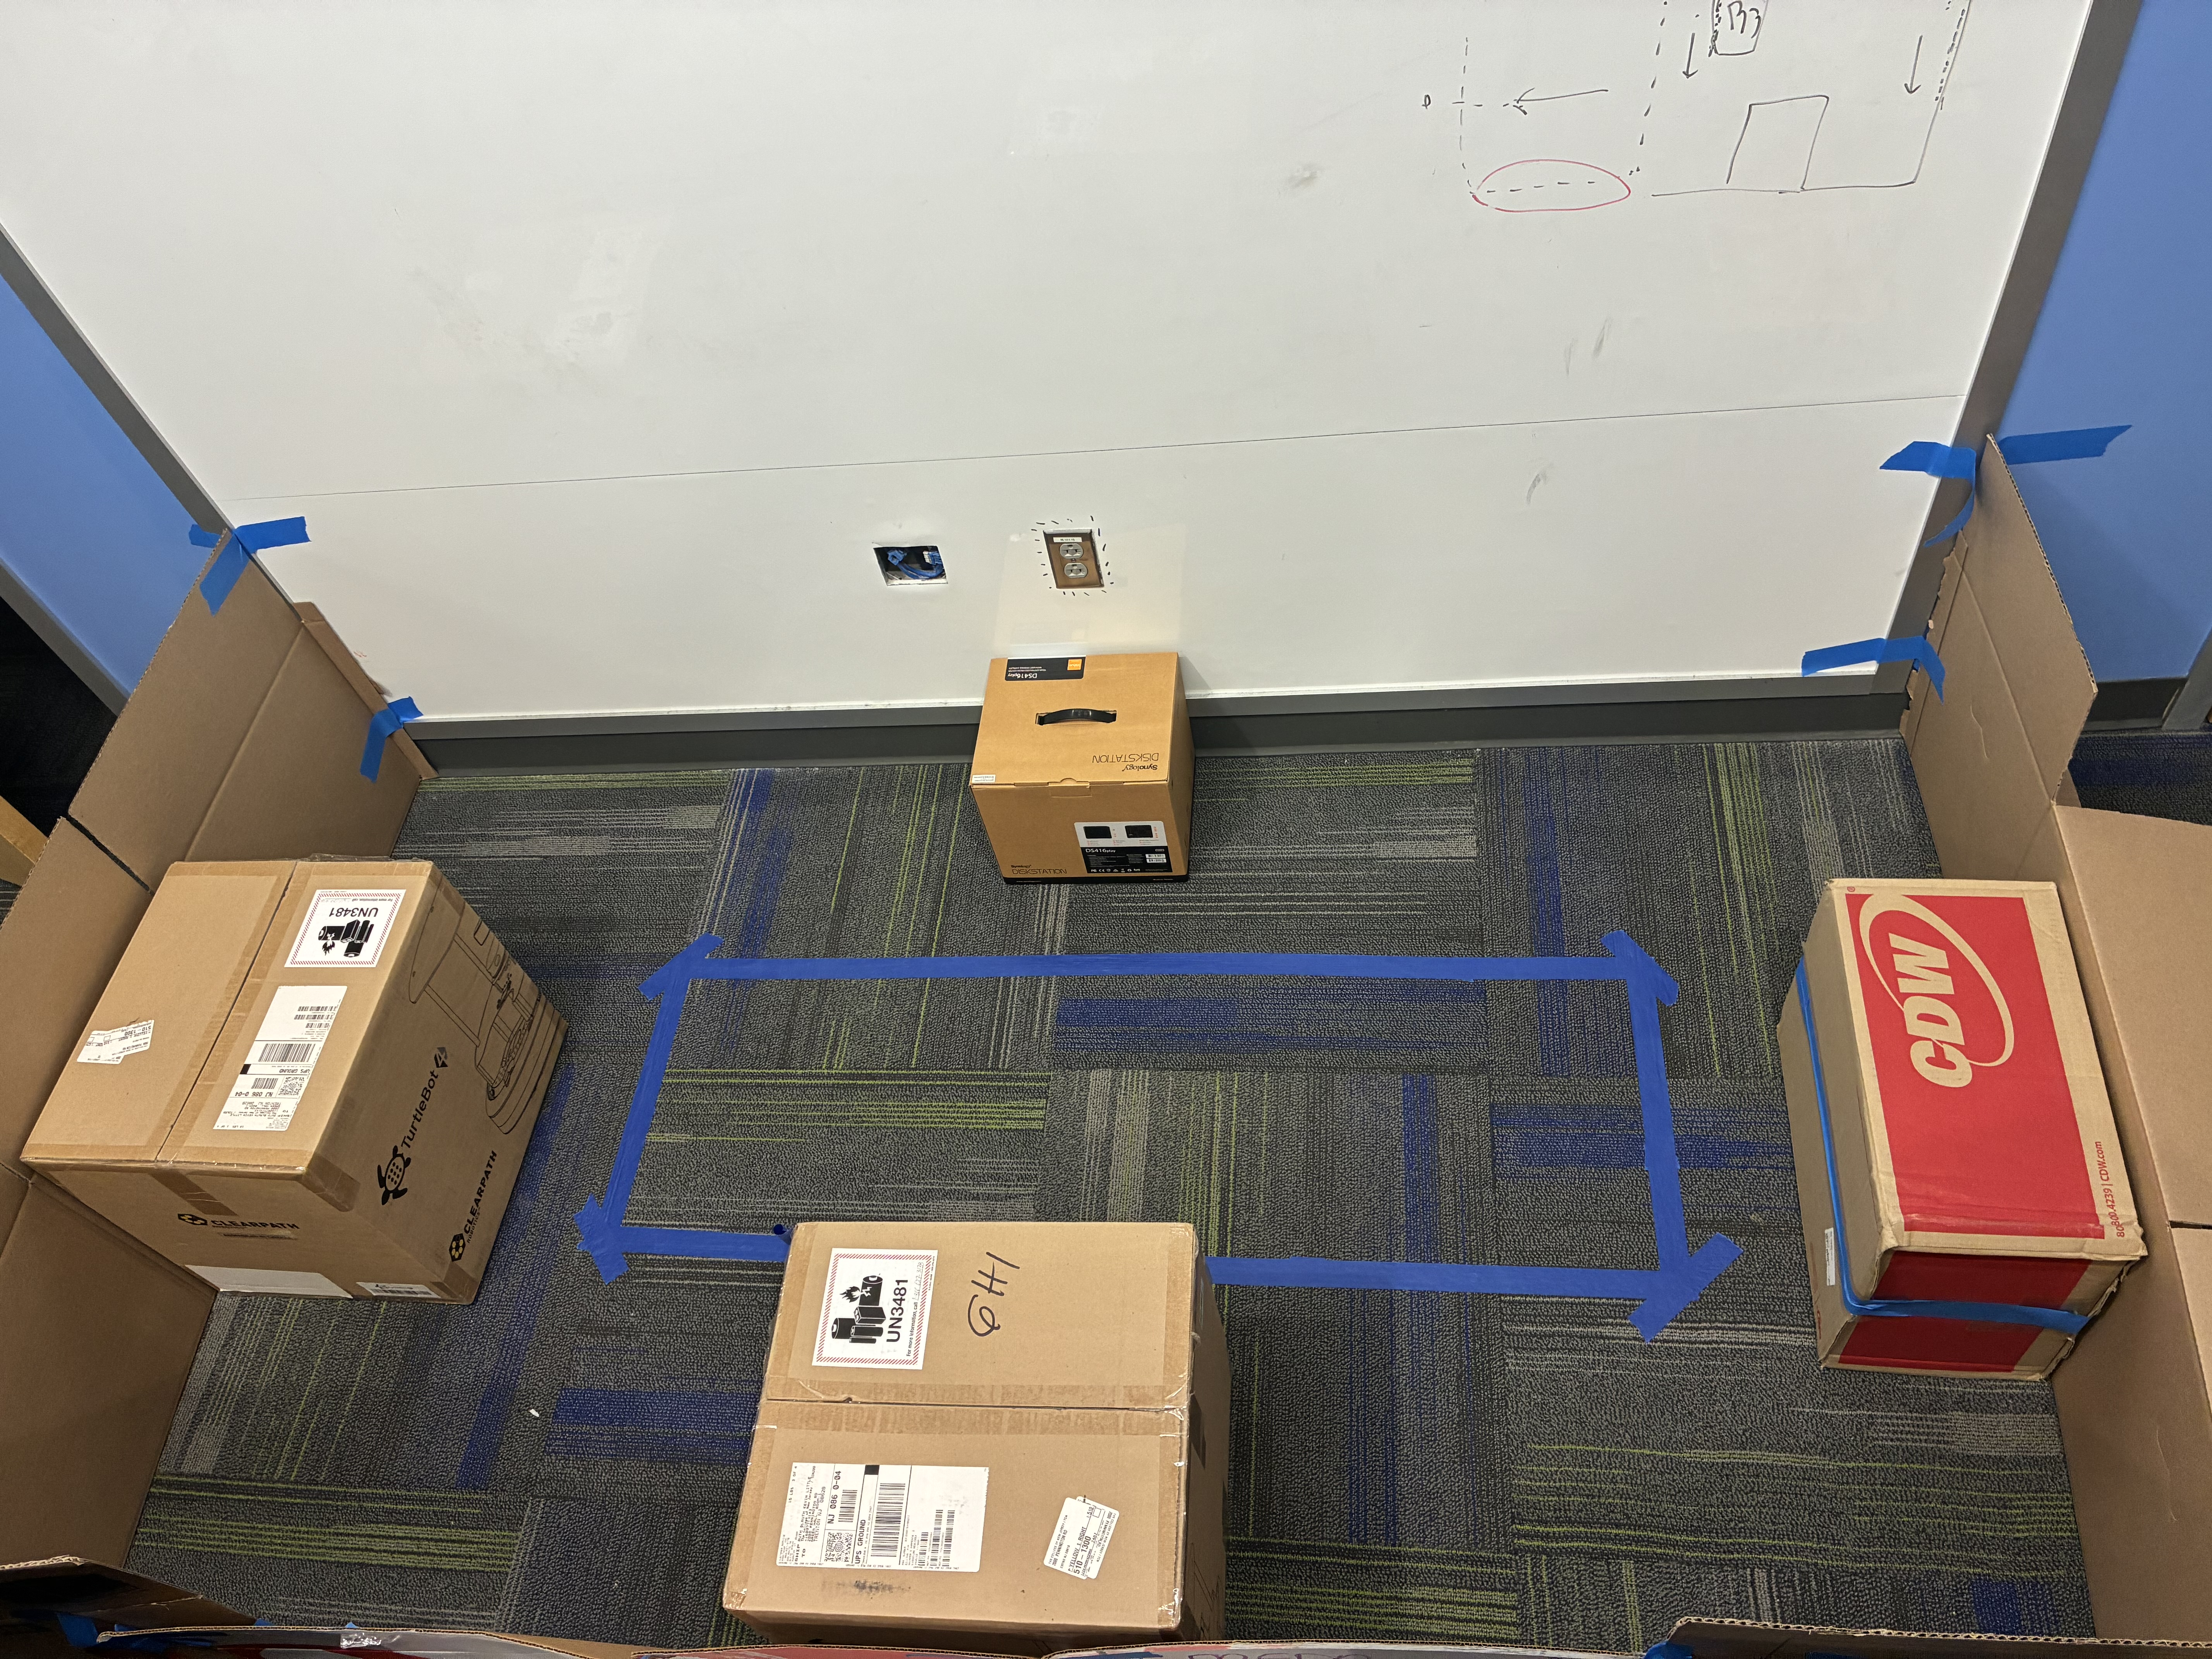
\includegraphics[width=0.45\columnwidth]{images/PictureOfMaze.jpg}}
        ~ % this will add a small gap between items
        \subfloat[Scaled reconstructed test environment]{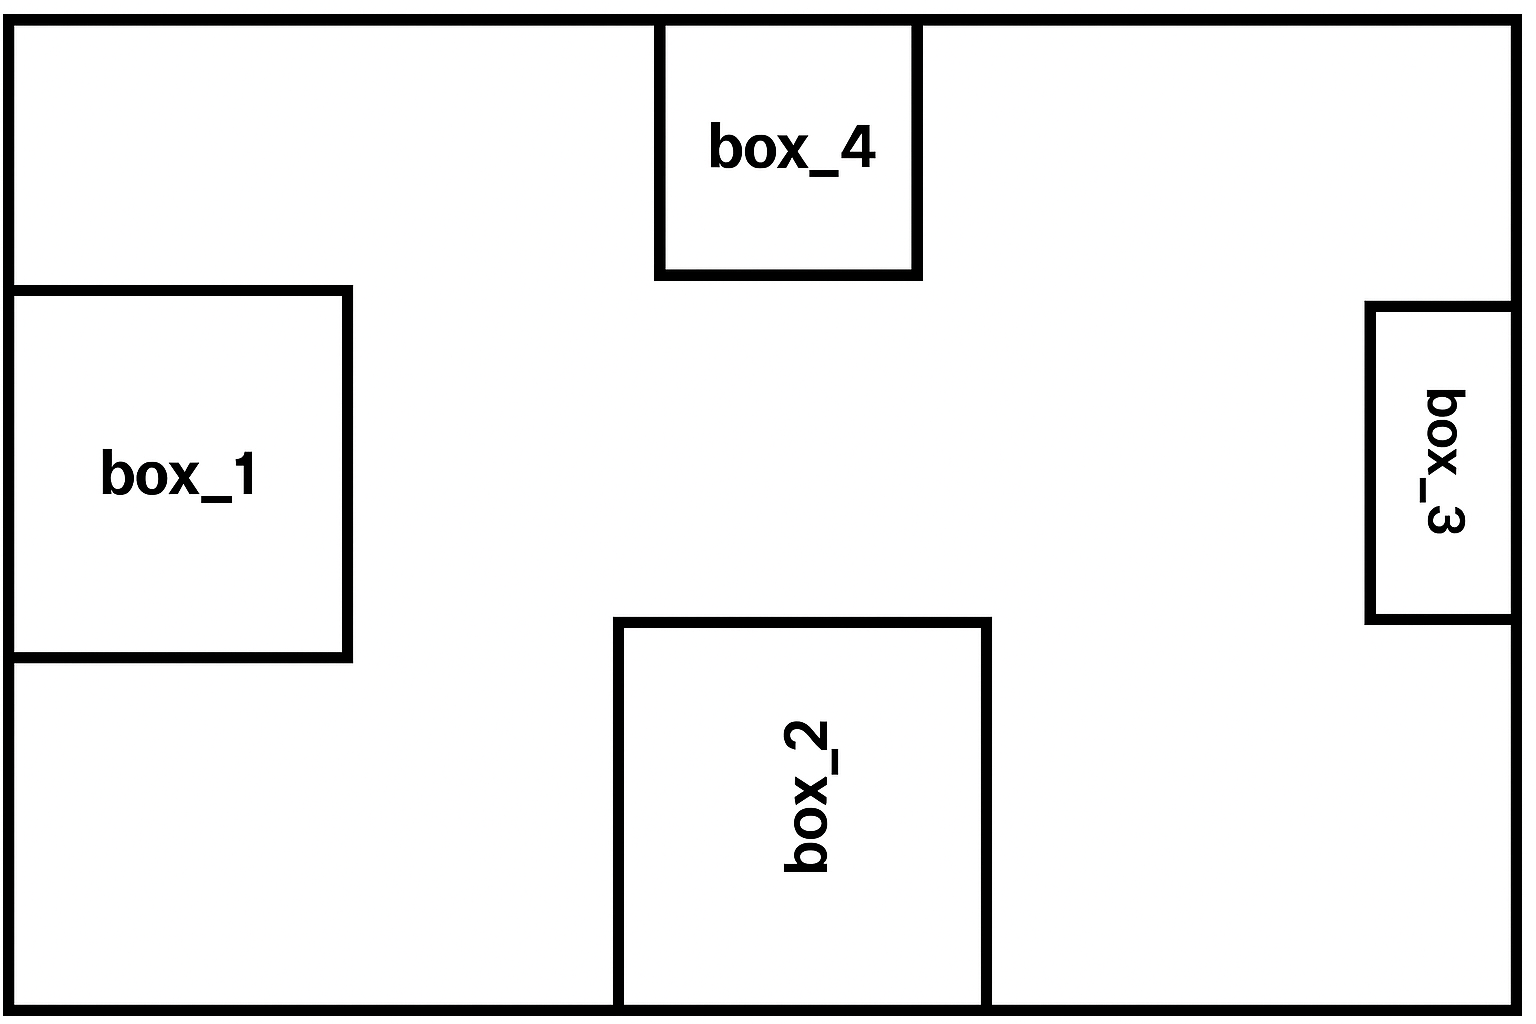
\includegraphics[width=0.45\columnwidth]{images/Black&Wite_testEnv.png}}
        % if you want to start a new row of figures, you can use two back slashes, i.e. \\
    \caption{Photographed and scaled reconstructed test environments.}
    \label{fig:subfigname}
\end{figure}

\subsubsection{Experiment procedure}
Ensuring that both SLAM algorithms were evaluated under the same conditions is one of the most critical requirements in comparative robotics research. A valid comparison requires eliminating as many external sources of variation as possible, so that any differences observed in the final maps can be attributed to the algorithms themselves rather than to inconsistencies in the testing procedure. This level of control is also essential for repeatability, allowing other researchers to reproduce the study and verify its results under identical conditions.

To achieve this level of consistency, I followed a strict, standardized experimental protocol for every trial. At the beginning of each run, the TurtleBot3 was placed in the same starting pose, aligned with the reference markers on the floor to minimize initial heading variation. Once positioned, I launched the designated SLAM algorithm, either SLAM Toolbox or Google Cartographer, and initiated the mapping process. Immediately afterward, I began manually teleoperating the robot along the predefined rectangular path marked with painter’s tape. The robot was driven at a constant linear velocity of 0.01 m/s, chosen specifically to reduce motion-induced noise and give the LiDAR sufficient time to gather stable measurements. Maintaining a fixed speed also prevented acceleration or deceleration effects from influencing scan matching or odometry drift.

Throughout the traversal, I maintained the same direction of motion and ensured the robot’s trajectory closely followed the taped path, maintaining its intended distance from each obstacle. Upon completing the full loop of the environment, I stopped the mapping process and saved the resulting occupancy grid using ROS2’s map server tools. This end-of-trial procedure ensured that each map was generated from an equivalent amount of spatial coverage and sensor data. The entire protocol was then repeated for the second SLAM algorithm under identical conditions. By controlling experimental variables such as starting pose, trajectory shape, robot speed, and map-saving procedure, the study ensured that SLAM Toolbox and Google Cartographer were evaluated fairly and that the resulting comparisons reflected actual algorithmic differences rather than inconsistent operational setups.

\begin{figure}[!ht] % this controls figure location. h is here, t is top, b is bottom. you can optionally use ! to enforce the layout, e.g. [!ht]
    \centering
        \subfloat[Saved map from Google Cartographer]{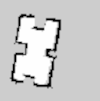
\includegraphics[width=0.45\columnwidth]{images/cartographer1_map.png}}
        ~ % this will add a small gap between items
        \subfloat[Saved map from SLAM Toolbox]{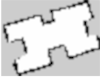
\includegraphics[width=0.45\columnwidth]{images/slam_toolbox1_map.png}}
        % if you want to start a new row of figures, you can use two back slashes, i.e. \\
    \caption{Saved maps from both SLAM algorithms after following the same path through the test environment.}
    \label{fig:subfigname}
\end{figure}

\subsubsection{Map Visual Comparison}
prior to performing any quantitative analysis, I first conducted a visual comparison of the maps generated by each SLAM algorithm. This step was crucial for identifying any obvious discrepancies or artifacts in the maps that could influence the subsequent quantitative evaluation.
This was the piont also where i noticesd that the mapps needed to be aligned and scaled to the ground truth before any quantitative analysis could be performed. To achieve this, 
I developed a custom Python script that utilized image processing techniques to align and scale the generated maps to match the ground truth dimensions. This involved identifying key features in the maps, such as the corners and edges of the boxes and extracting their exact pixel coordinates. 
Working at the pixel level was essential because all subsequent transformations and error calculations depend on spatial relationships expressed in pixels. Without converting these features into precise pixel measurements, the system would not be able to correctly align the maps, compute differences, or quantify mapping accuracy.

\subsubsection{Quantitative Analysis}
At this point in my project, I had understood from looking at the maps that I had saved from both SLAM algorithims that I needed to center the images and scale them to a common resolution before I could perform any quantitative analysis.
To do this, I wrote a custom Python script that used image processing techniques to align and scale the generated maps to match the ground truth dimensions. This involved identifying key features in the maps, such as the corners and edges of the boxes, and extracting their exact pixel coordinates. 
Once the maps were aligned and scaled, I proceeded to compute quantitative error metrics to evaluate the mapping accuracy of each SLAM algorithm. The primary metrics I focused on were per-pixel map error, variance, and correlation with the ground truth. 
Per-pixel map error was calculated by comparing the occupancy values of each pixel in the generated map to the corresponding pixel in the ground truth map. This provided a detailed measure of how closely each algorithm's map matched the actual environment. Variance was computed to assess the consistency of the mapping results across multiple trials for each algorithm. 
A lower variance indicated that the algorithm produced more consistent maps under the same conditions. Finally, I calculated the correlation coefficient between the generated maps and the ground truth to quantify the overall similarity in spatial structure. A higher correlation coefficient indicated a closer match between the generated map and the ground truth. 

\subsubsection{Mean Squared Error (MSE) Comparison}
This is a pear reviwed method that is commonly used to measure the average squared difference between the estimated values and the actual value. In this case, the estimated values are the pixel values from the SLAM generated maps, and the actual values are the pixel values from the ground truth map.
This peer-reviewed method is commonly used to measure the average squared difference between estimated and actual values. In this context, the calculated values are the pixel intensities from the SLAM-generated maps, and the exact values are those from the ground-truth map. 
In the literature, the authors who originally applied this technique used pixel-wise comparison metrics, such as MSE, RMSE, and correlation, to objectively evaluate SLAM performance across repeated mapping trials. 
Their process involved converting each map into a uniform pixel grid, extracting corresponding pixel values from the estimated and ground-truth maps, and then computing statistical error metrics that quantify how closely the SLAM output matches the actual environment. By doing so, they were able to derive numerical measures of accuracy, consistency, and deviation, rather than relying solely on visual inspection[5].

\begin{figure}[!ht] % this controls figure location. h is here, t is top, b is bottom. you can optionally use ! to enforce the layout, e.g. [!ht]
    \centering
        \subfloat[Root mean squared error (RMSE)]{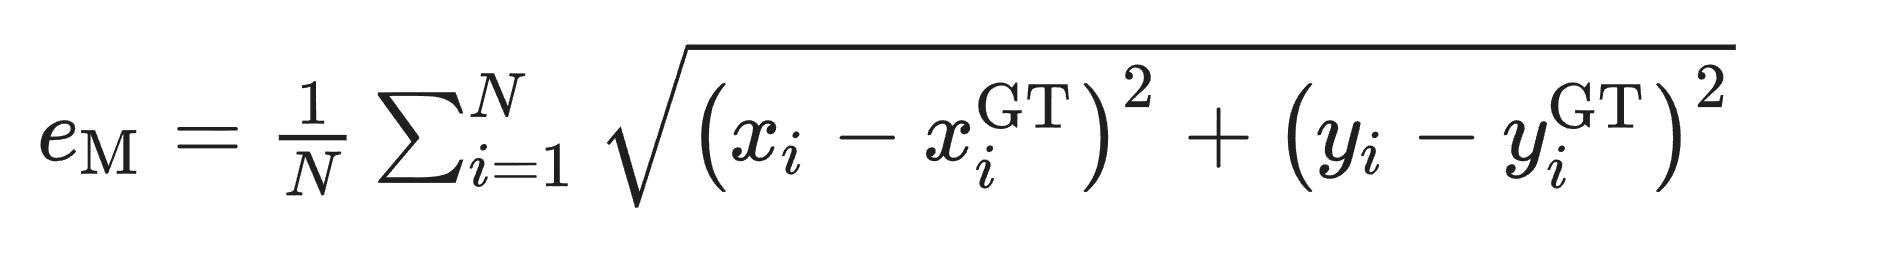
\includegraphics[width=0.45\columnwidth]{images/RMSE.png}}
        % if you want to start a new row of figures, you can use two back slashes, i.e. \\
    \caption{Root mean squared error (RMSE) calculation between algorithims and ground-truth maps.}
    \label{fig:subfigname}
\end{figure}

In the same way, I applied this method in my study by first resizing all maps to a fixed pixel dimension, identifying and aligning key features, and then comparing pixel values directly between the SLAM Toolbox map, Cartographer map, and the drawn ground-truth map. 
Once the maps were normalized and aligned, I computed the same peer-reviewed metrics: the average squared pixel error, the variance, the MSE, and the correlation between the estimated and ground-truth maps. Using this approach allowed me to quantify the extent to which each algorithm deviated from the ground truth under identical test conditions. 
This objective, pixel-based comparison method provided a rigorous and repeatable way of determining which SLAM algorithm produced a map more faithful to the actual layout, ensuring that the conclusions of my study were supported by measurable, statistical evidence rather than subjective observation.

\begin{figure}[!ht] % this controls figure location. h is here, t is top, b is bottom. you can optionally use ! to enforce the layout, e.g. [!ht]
    \centering
        \subfloat[Root mean squared error (RMSE)]{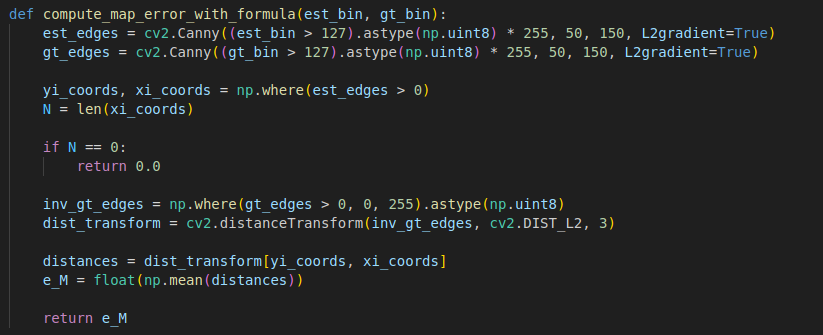
\includegraphics[width=0.45\columnwidth]{images/RMSE_code.png}}
        % if you want to start a new row of figures, you can use two back slashes, i.e. \\
    \caption{Root mean squared error (RMSE) calculation based on the Python code snippet.}
    \label{fig:subfigname}
\end{figure}

\subsubsection{Correlation and Variance Comparison}
In this project, another important quantitative analysis involved comparing the correlation and variance between the generated SLAM maps and the ground-truth map. Correlation measures the strength and direction of the linear relationship between two sets of pixel values in this case, the pixel intensities of the estimated map and the corresponding pixel intensities of the ground-truth map. The method used to compute this statistic was the Pearson correlation coefficient, a peer-recognized and widely used approach for assessing similarity between two numerical datasets. 
The Pearson correlation coefficient is calculated using the formula:
\begin{equation}
    r = \frac{\sum (X_i - \bar{X})(Y_i - \bar{Y})}{\sqrt{\sum (X_i - \bar{X})^2 \sum (Y_i - \bar{Y})^2}}
    \label{eq:}
\end{equation}
    
where \(X_i\) and \(Y_i\) are the pixel values from the SLAM-generated map and the ground-truth map, respectively, and \(\bar{X}\) and \(\bar{Y}\) are their respective means. The resulting coefficient \(r\) ranges from -1 to 1, where values close to 1 indicate a strong positive correlation, values close to -1 indicate a strong negative correlation, and values near 0 suggest no linear relationship.

A high positive Pearson correlation between the SLAM output and the ground-truth map suggests that the two maps change together consistently: when the ground-truth map shows an obstacle or structural boundary (represented by higher pixel values), the SLAM-generated map also reflects a similar intensity pattern at the corresponding location. This is an indication that the algorithm accurately captured the overall structure of the environment. Conversely, a weak or near-zero correlation indicates that the estimated map does not reliably follow the spatial patterns of the ground-truth map, implying structural mismatches or inconsistent mapping performance.

Variance provides a complementary perspective by measuring the spread or dispersion of pixel values within the generated map. In this context, variance reflects how much the pixel intensities fluctuate across the map's occupied and unoccupied regions. Lower variance indicates that the estimated map is more uniform and stable, which often suggests that the SLAM algorithm consistently detected obstacles and free space. Higher variance, on the other hand, may indicate noise, irregular edges, or inconsistent detection of environmental features. When interpreted alongside Pearson correlation, variance helps determine not only how well the generated map aligns with the ground truth, but also how stable, clean, and consistent the algorithm’s mapping output is across the entire image.

\section{Observatuions and Results}
\subsection{Qualitative Observations}

What we are seeing in these images is an overlay of the generated maps from both SLAM algorithms on top of the ground truth map. This visual comparison allows us to qualitatively assess how well each algorithm captured the structure of the environment. In the left image, we see the maps produced by Google Cartographer, while the right image shows those generated by SLAM Toolbox.
From the overlay, we can observe several key differences between the two algorithms. The Cartographer maps appear to have more distortion and misalignment with the ground truth, particularly around the corners and edges of the boxes. This suggests that Cartographer may have struggled with accurately mapping the environment, leading to discrepancies in the representation of obstacles. In contrast, the SLAM Toolbox maps show a closer alignment with the ground truth, with fewer distortions and a more accurate depiction of the boxes' shapes and positions. This indicates that SLAM Toolbox was more effective at capturing the true layout of the environment, resulting in a more faithful representation. Overall, this qualitative comparison highlights the strengths and weaknesses of each SLAM algorithm in terms of mapping accuracy and consistency.
\begin{figure}[h!] % this controls figure location. h is here, t is top, b is bottom. you can optionally use ! to enforce the layout, e.g. [!ht]
    \centering
        \subfloat[Cartographer maps overlaid on GT]{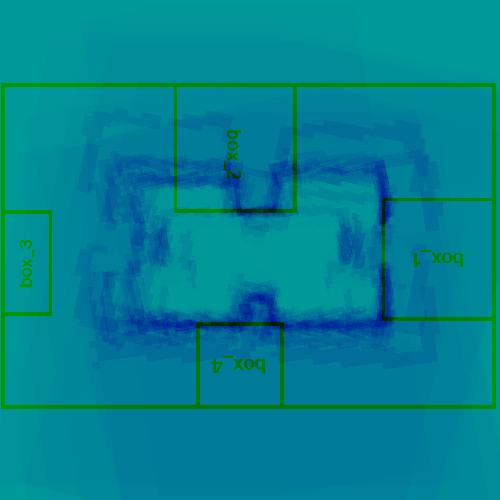
\includegraphics[width=0.45\columnwidth]{images/overlay_cartographer_avg_vs_groundtruth.png}}
        ~ % this will add a small gap between items
        \subfloat[SLAM Toolbox maps overlaid on GT]{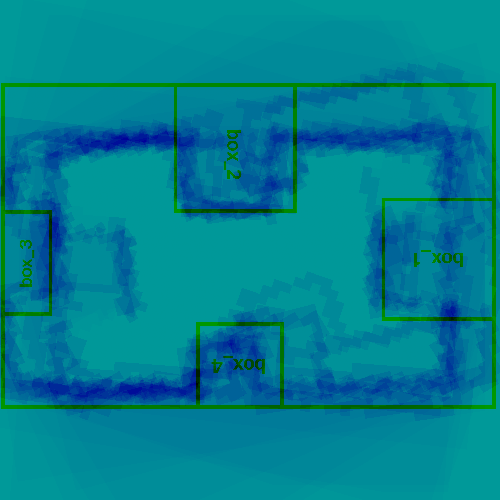
\includegraphics[width=0.45\columnwidth]{images/overlay_slam_avg_vs_groundtruth.png}}
        % if you want to start a new row of figures, you can use two back slashes, i.e. \\
    \caption{Overlay of generated maps on the Ground Truth (GT) for qualitative comparison.}
    \label{fig:subfigname}
\end{figure}

\subsection{Quantitative Observations}
\begin{table}[h!]
\centering
\caption{Quantitative Comparison of Cartographer and SLAM Toolbox}
\begin{tabular}{lcccc}
\hline
\textbf{} & \textbf{Cartographer (px)} & \textbf{Cartographer (cm)} & \textbf{SLAM Toolbox (px)} & \textbf{SLAM Toolbox (cm)} \\
\hline
\textbf{Mean Error}      & 25.227 & 126.134 & 19.294 & 96.468 \\
\textbf{Variance}        & 5.517  & 137.918 & 7.207  & 180.167 \\
\textbf{MSE}             & 641.909 & 16047.729 & 379.448 & 9486.196 \\
\textbf{RMSE}            & 25.336 & 126.680 & 19.479 & 97.397 \\
\textbf{Correlation}     & 0.246 & -- & 0.169 & -- \\
\hline
\end{tabular}
\label{tab:slam_comparison}
\end{table}

Table 1 presents a quantitative comparison of mapping performance between Google Cartographer and SLAM Toolbox using several key evaluation metrics: Mean Error, Variance, Mean Squared Error (MSE), Root Mean Squared Error (RMSE), and Pearson Correlation with the ground-truth map. These metrics were computed in pixel space and also converted to centimeters for practical interpretation of mapping accuracy in the physical environment. The combination of these values allows for a multidimensional assessment of each algorithm’s precision, consistency, and structural similarity to the actual map.

Overall, the results show that SLAM Toolbox outperformed Cartographer in nearly all core accuracy metrics. SLAM Toolbox achieved a lower Mean Error of 19.294 pixels (96.468 cm) compared to Cartographer’s 25.227 pixels (126.134 cm), indicating that its generated map more closely matched the actual layout on average. Although SLAM Toolbox exhibited a slightly higher Variance (7.207 px vs. 5.517 px), this difference is relatively small. It suggests that while SLAM Toolbox was more accurate on average, its pixel-level deviations were somewhat more spread out. In practical terms, SLAM Toolbox achieved better accuracy but with only mildly increased variability, an acceptable trade-off in most mapping applications.

The MSE and RMSE values further reinforce this pattern. SLAM Toolbox produced a substantially lower MSE (379.448 px) than Cartographer (641.909 px), meaning that the squared pixel-wise differences between SLAM Toolbox’s map and the ground truth were significantly smaller overall. The RMSE results 19.479 px for SLAM Toolbox versus 25.336 px for Cartographer—show the same trend when error magnitude is returned to a linear scale. These metrics together demonstrate not only improved average accuracy but also a more reliable reconstruction of the environment's structural features.

The correlation metric, however, presents an interesting nuance. The cartographer achieved a higher Pearson correlation coefficient (0.246) than SLAM Toolbox (0.169), indicating that its pixel intensities exhibited a slightly stronger linear relationship with those of the ground-truth map. While this suggests that Cartographer preserved specific structural gradients more faithfully, correlation alone does not directly measure absolute accuracy only similarity in intensity patterns. When interpreted alongside the substantially lower error values produced by SLAM Toolbox, the higher correlation from Cartographer does not outweigh the more meaningful improvements SLAM Toolbox demonstrated across Mean Error, MSE, and RMSE.

Taken together, these findings indicate that SLAM Toolbox generated maps that were closer to the ground truth in absolute geometric accuracy, even though Cartographer maintained a slightly stronger linear relationship at the pixel level with the reference map. In practice, the lower Mean Error and RMSE values from SLAM Toolbox offer more reliable evidence of superior mapping performance. 


\begin{figure}[h!]
\centering
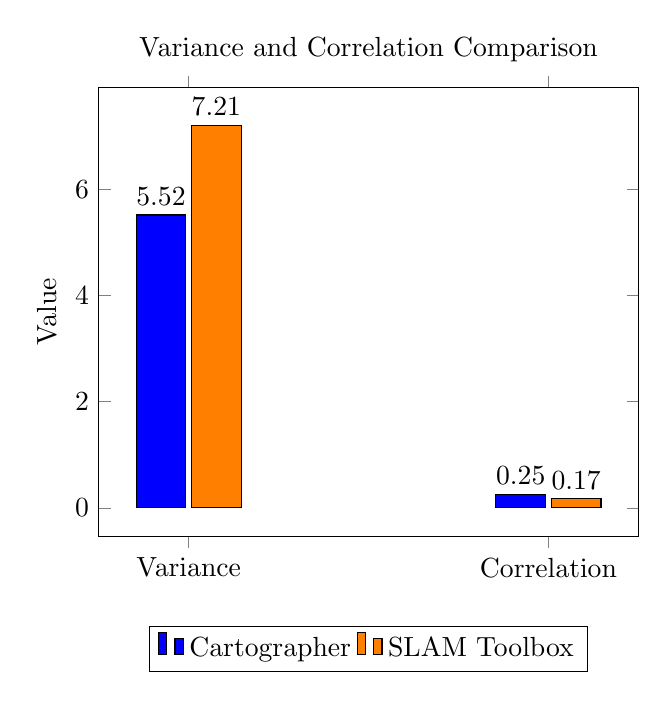
\begin{tikzpicture}
\begin{axis}[
    ybar,
    bar width=18pt,
    enlarge x limits=0.25,
    ylabel={Value},
    symbolic x coords={Variance,Correlation},
    xtick=data,
    nodes near coords,
    legend style={at={(0.5,-0.2)},anchor=north,legend columns=-1},
    title={Variance and Correlation Comparison}
]

\addplot[fill=blue] coordinates {
    (Variance,5.517)
    (Correlation,0.246)
};
\addlegendentry{Cartographer}

\addplot[fill=orange] coordinates {
    (Variance,7.207)
    (Correlation,0.169)
};
\addlegendentry{SLAM Toolbox}

\end{axis}
\end{tikzpicture}
\caption{Bar chart comparing Variance and Correlation for both SLAM algorithms.}
\end{figure}

\begin{figure}[h!]
\centering
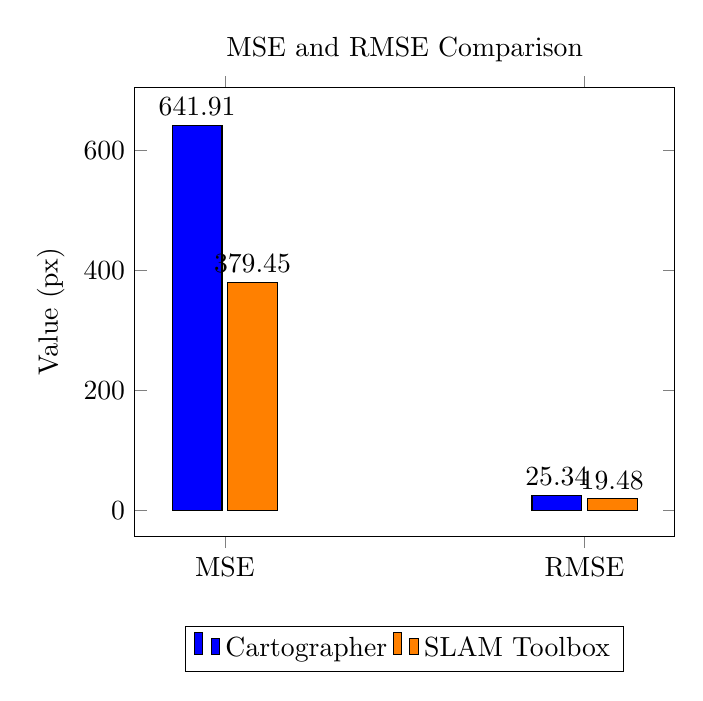
\begin{tikzpicture}
\begin{axis}[
    ybar,
    bar width=18pt,
    enlarge x limits=0.25,
    ylabel={Value (px)},
    symbolic x coords={MSE,RMSE},
    xtick=data,
    nodes near coords,
    legend style={at={(0.5,-0.2)},anchor=north,legend columns=-1},
    title={MSE and RMSE Comparison}
]

\addplot[fill=blue] coordinates {
    (MSE,641.909)
    (RMSE,25.336)
};
\addlegendentry{Cartographer}

\addplot[fill=orange] coordinates {
    (MSE,379.448)
    (RMSE,19.479)
};
\addlegendentry{SLAM Toolbox}

\end{axis}
\end{tikzpicture}
\caption{Bar chart comparing MSE and RMSE for both SLAM algorithms.}
\end{figure}

\subsection{Discussion of Results}
The quantitative results from this study provide a clear comparison of mapping performance between Google Cartographer and SLAM Toolbox. Across multiple key metrics, SLAM Toolbox consistently outperformed Cartographer in terms of absolute accuracy, as evidenced by lower Mean Error, MSE, and RMSE values. These findings suggest that SLAM Toolbox is more effective at reconstructing the true layout of the environment, producing maps that are closer to the ground truth.
The slightly higher Variance observed in SLAM Toolbox indicates that while it achieved better average accuracy, its pixel-level deviations were somewhat more spread out. However, this trade-off is generally acceptable in mapping applications, as the overall accuracy gains outweigh the minor increase in variability.

The correlation results present an interesting nuance, with Cartographer achieving a higher Pearson correlation coefficient than SLAM Toolbox. This suggests that Cartographer preserved specific structural gradients more faithfully, but correlation alone does not directly measure absolute accuracy. When interpreted alongside the substantially lower error values produced by SLAM Toolbox, the higher correlation from Cartographer does not outweigh the more meaningful improvements SLAM Toolbox demonstrated across Mean Error, MSE, and RMSE.

\section{Conclusion and Future Work}
\subsection{Summary of Findings}
This study conducted a comparative analysis of two widely used SLAM algorithms, Google Cartographer and SLAM Toolbox, using a controlled physical environment constructed from cardboard boxes. The TurtleBot3 platform equipped with a 2D LiDAR sensor was manually teleoperated through the environment, and maps were generated using both algorithms under identical conditions. A custom Python pipeline was developed to align the generated maps with the ground truth and compute quantitative error metrics, including Mean Error, Variance, MSE, RMSE, and Pearson Correlation. The results demonstrated that SLAM Toolbox consistently outperformed Cartographer in terms of absolute accuracy, achieving lower Mean Error, MSE, and RMSE values. Although SLAM Toolbox exhibited slightly higher Variance, this trade-off was deemed acceptable given the overall accuracy gains. The correlation results indicated that while Cartographer preserved structural gradients more faithfully, this did not compensate for its higher error metrics.

\subsection{Threats to Validity}

As with any empirical study involving physical robot systems, several factors may influence the
interpretation and generalizability of the results. These potential threats to validity do not diminish
the findings but instead highlight areas where additional work may further strengthen the reliability
of the conclusions.

One internal concern is the reliance on manual teleoperation to guide the
TurtleBot3 along the predefined path. Although speed and trajectory were kept as consistent as
possible across all trials, slight variations in robot motion or operator input may introduce minor
differences in the LiDAR data that each SLAM algorithm receives. Additionally, environmental
factors such as lighting conditions, floor reflections, or slight shifts in the cardboard obstacles
could affect sensor readings. Care was taken to minimize these variables, but they remain inherent
sources of noise in physical experiments.

The controlled cardboard Maze environment was intentionally designed
to simplify measurement and provide clear geometric features for evaluation. However, real-world
environments often exhibit far more variability, including irregular surfaces, dynamic objects, and
unstructured layouts. As a result, the performance of SLAM Toolbox and Google Cartographer in
this study may not fully represent their behavior in more complex or dynamic settings. Further
experiments across diverse environments would be necessary to extend the conclusions.

The quantitative metrics used in this study, including per-pixel map
error, variance, MSE, RMSE, and Pearson correlation, provide meaningful insight into structural
accuracy. However, these metrics operate primarily in pixel space and do not capture all aspects of
SLAM performance. For example, global consistency, loop closure reliability, and long-term
Trajectory drift cannot be fully evaluated solely from occupancy grid comparisons. Thus, while the
metrics offer a strong foundation for comparing map quality, they represent only one dimension of
SLAM system evaluation.

One way to strengthen the validity of these findings is to
repeat the experiments in a simulated environment such as Gazebo. Gazebo is a high-fidelity
A physics simulator commonly used in robotics research, capable of accurately modeling robot
kinematics, sensor noise, LiDAR scans, and obstacle interactions. By recreating the Maze in
simulation and running both SLAM algorithms under identical digital conditions, it would be
possible to verify whether the trends observed in the physical experiments persist in a noise-
controlled environment. Simulation also removes operator-dependent variability, ensuring that the
robot follows precisely the same trajectory for each trial. If the results in Gazebo align with those
collected in the real world, this would provide substantial additional evidence supporting the robustness
of the conclusions drawn in this study.

Overall, acknowledging these threats to validity is an essential part of establishing the scope and
limitations of the present work. While every effort was made to control experimental conditions
and perform a rigorous comparison, future studies incorporating simulation, dynamic environments,
Autonomous navigation pipelines would provide a more comprehensive assessment of SLAM
algorithm performance.


\subsection{Conclusion of Research}
The results of this study demonstrate the importance of selecting an appropriate SLAM algorithm
when developing mobile robotic systems that depend on accurate and repeatable environmental
representation. Although both Google Cartographer and SLAM Toolbox are widely used within the
In the ROS2 ecosystem, their performance in this controlled evaluation showed clear and measurable
differences. Across the primary quantitative metrics Mean Error, MSE, RMSE, and Variance
SLAM Toolbox consistently produced maps that more closely matched the physical dimensions of
the Maze. These findings suggest that SLAM Toolbox may be the more suitable choice in robotic
applications where precise geometric reconstruction is essential, such as autonomous navigation,
manipulation near obstacles, or environments requiring reliable loop-closure detection.

Beyond identifying which algorithm performed better in this specific environment, the study also
highlights the broader value of using quantitative metrics to evaluate SLAM performance. Visual
inspection alone is insufficient for assessing subtle distortions, scale drift, or misalignment in
occupancy grid maps. By normalizing, aligning, and comparing maps at the pixel level, it becomes
possible to capture structural differences that would otherwise remain hidden. This reinforces the
need for objective evaluation frameworks in robotics research, particularly when algorithmic
performance may directly influence safety, autonomy, or long-term deployment stability.

While SLAM Toolbox demonstrated superior mapping accuracy, the study also revealed
interesting nuances in algorithm behavior. Cartographer achieved a slightly higher Pearson
correlation coefficient with the ground truth, indicating that its pixel intensities maintained a
stronger linear relationship with the reference map. However, correlation alone does not fully
capture geometric accuracy; it reflects similarity in intensity patterns rather than absolute spatial
correctness. When interpreted alongside the substantially lower error metrics produced by SLAM
Toolbox, the higher correlation does not outweigh the overall mapping advantages observed in
SLAM Toolbox. Together, these results provide a balanced perspective on the strengths and
limitations of each SLAM framework and highlight the importance of multi-metric analysis when
evaluating SLAM algorithms.

This research also underscores the significance of carefully controlling experimental conditions.
By using a repeatable path, fixed velocity, identical starting pose, and a precisely measured
physical environment, it was possible to ensure that each SLAM algorithm was evaluated under
truly comparable conditions. This level of experimental rigor is essential for drawing reliable
conclusions about SLAM performance. The methodology developed in this study including the
alignment, normalization, and pixel-based comparison pipeline can serve as a foundation for
future work evaluating not only these two algorithms but also other SLAM frameworks or sensor
configurations.

Looking forward, the results obtained here represent an initial step toward a broader investigation
into robustness and long-term autonomy in mobile robots. More complex environments involving
dynamic obstacles, irregular geometry, or multi-room layouts would provide additional insight into
how each algorithm scales beyond controlled conditions. Likewise, repeating the study in simulation
(e.g., Gazebo) would offer a noise-controlled setting to validate the consistency of the findings and
remove operator-induced variability. Exploring each algorithm's ability to handle loop closure,
global pose correction, and multi-session mapping would further expand understanding of their
capabilities in real-world scenarios. Ultimately, by establishing a rigorous and repeatable evaluation
framework, this study contributes not only a direct comparison of Cartographer and SLAM Toolbox
but also a methodology that can support ongoing research in mapping, localization, and navigation
within the robotics community.

\subsection{Suggestions for Future Work}
Building on the findings of this study, several avenues for future research can be pursued to further enhance our understanding of SLAM algorithm performance. One potential direction is to evaluate the algorithms in more complex and dynamic environments, such as outdoor settings or indoor spaces with moving obstacles. This would provide insights into how well each algorithm adapts to changing conditions and handles real-world challenges. Additionally, investigating the impact of different sensor configurations, such as varying LiDAR resolutions or incorporating additional sensors like cameras or IMUs, could shed light on how sensor fusion influences mapping accuracy. Another important area for future work is to explore the algorithms' capabilities in addressing higher-level challenges, such as loop closure and long-term autonomy. Implementing scenarios where the robot revisits previously mapped areas would test the algorithms' ability to recognize and correct accumulated drift. Finally, conducting user studies to assess the practical usability and integration of these SLAM frameworks within broader robotic systems could provide valuable feedback for developers.


%

% the environments 'definition', 'lemma', 'proposition', 'corollary',
% 'remark', and 'example' are defined in the LLNCS documentclass as well.
%


%
% ---- Bibliography ----
%
% List of references does not count toward your report. 
% Make sure this pages starts from page number 21 (in case of capstone).
\newpage
%
% BibTeX users may specify bibliography style 'ieee'.
% References will then be sorted and formatted in the correct style.
%
% See mybibliography.bib file for details.
\bibliographystyle{ieee}
\bibliography{mybibliography}
%
% ----------------------------------------------------------------------
% Alternatively, you can manually add bibitems in .tex file like below.
% However, this method is *strongly discouraged*.
%
% \begin{thebibliography}{8}
% \bibitem{ref_article1}
% Author, F.: Article title. Journal \textbf{2}(5), 99--110 (2016)

% \bibitem{ref_lncs1}
% Author, F., Author, S.: Title of a proceedings paper. In: Editor,
% F., Editor, S. (eds.) CONFERENCE 2016, LNCS, vol. 9999, pp. 1--13.
% Springer, Heidelberg (2016). \doi{10.10007/1234567890}

% \bibitem{ref_book1}
% Author, F., Author, S., Author, T.: Book title. 2nd edn. Publisher,
% Location (1999)

% \bibitem{ref_proc1}
% Author, A.-B.: Contribution title. In: 9th International Proceedings
% on Proceedings, pp. 1--2. Publisher, Location (2010)

% \bibitem{ref_url1}
% LNCS Homepage, \url{http://www.springer.com/lncs}. Last accessed 4
% Oct 2017
% \end{thebibliography}
% ----------------------------------------------------------------------
%

\end{document}
